\section{Project Management}

\subsection{Version Control}

Packet Courier was developed using Git\cite{git} as a version control system and the code repository is hosted on
GitHub\cite{github, packet_courier} at \url{https://github.com/thelukethorpe/packet_courier}. There is no special
reason for either of these choices; they are simply industry standards being used for a project that doesn't
innately demand bespoke tooling (unlike data-heavy ventures such as game development, which might benefit from a tool
like Perforce\cite{perforce, perforce_vs_git}).

\subsection{Ticket Tracking}

GitHub Issues\cite{github_issues} powers Packet Courier's ticket tracking. Tickets, or \emph{issues}, as per the
GitHub nomenclature, are categorised based on one or more of the following custom tags:
\begin{itemize}
    \item \textbf{Bug:} \emph{Something isn't working.}
    \item \textbf{CI:} \emph{Change to pipeline.}
    \item \textbf{Documentation:} \emph{Improvements or additions to documentation.}
    \item \textbf{Feature:} \emph{New feature or request.}
    \item \textbf{Optimization:} \emph{Improvements in performance.}
    \item \textbf{Refactor:} \emph{Tech-debt, structural change of quality-of-life improvement.}
    \item \textbf{Testing:} \emph{Improvements or additions to test suite.}
    \item \textbf{Won't Fix:} \emph{This will not be worked on.}
\end{itemize}

Issues are further organised using a Kanban board\cite{kanban_board}. As the \emph{documentation} tag suggests,
this board is not only used for development purposes, in fact, it has been used to help manage the project
holistically, including the writing of this very report, as shown in
Figure~\ref{fig:chapter_4_implementation-github_kanban_board}.

\begin{figure}[!h]
    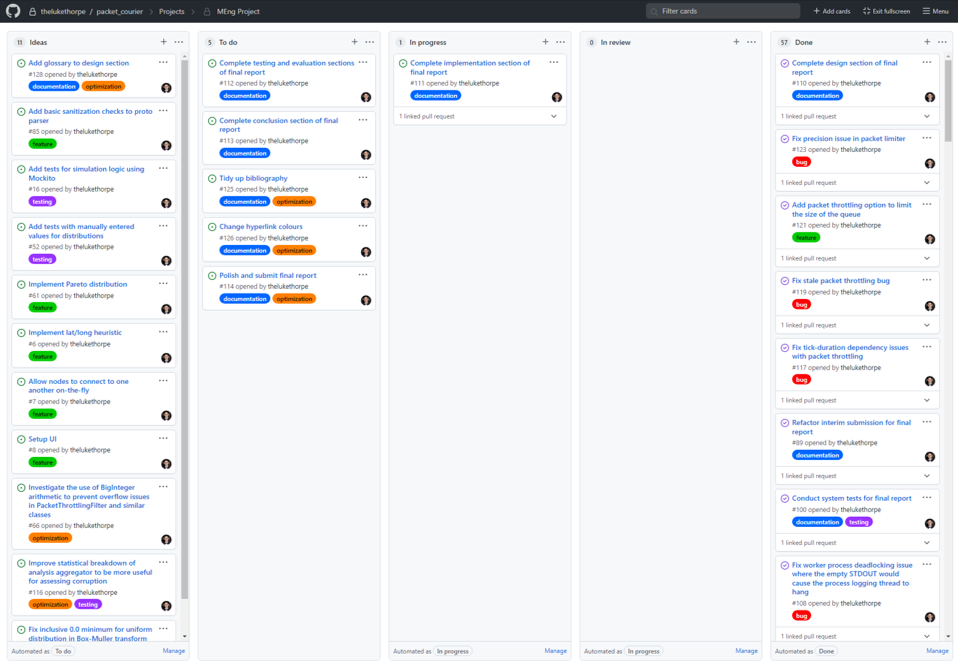
\includegraphics[width=\textwidth]{images/chapter_4_implementation/github_kanban_board}
    \centering~\caption{Packet Courier's Project Kanban Board\cite{packet_courier}.}
    \label{fig:chapter_4_implementation-github_kanban_board}
\end{figure}

Pull-requests are opened for every merge to the \texttt{main} branch and linked to the associated ticket number.
Branches are named with a uniform and consistent structure, prefixed by the issue number followed by a brief subtitle
of the ticket delimited by hyphens. Despite being an individual project, this repository has been maintained to
industry standards of software engineering practices for organisational reasons, and has in turn benefited massively
from it.

\begin{figure}[!h]
    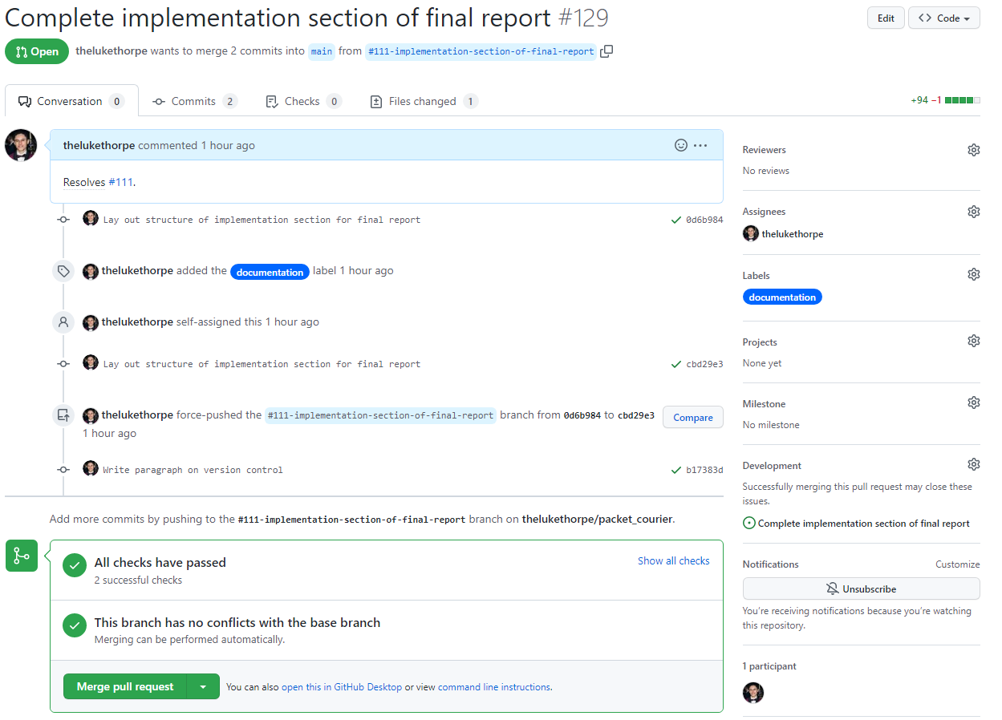
\includegraphics[width=\textwidth]{images/chapter_4_implementation/github_pull_request}
    \centering~\caption{An example of a pull-request in the Packet Courier repository\cite{packet_courier}.}
    \label{fig:chapter_4_implementation-github_pull_request}
\end{figure}

\newpage

\subsection{Programming Languages}

Java 8\cite{java_8} was chosen as the foundational language for Packet Courier due to:
\begin{itemize}
    \item Its excellent breadth of supported platforms\cite{java_8_support}, which lends itself well to objective 4.a).
    \item The vast number of popular and easily importable libraries available to it\cite{java_relevance}.
    \item Its object-oriented nature, which maps nicely onto the abstract semantics laid out in the design section.
    \item Its relatively high levels of time-efficiency, as shown in
    Figure~\ref{fig:chapter_4_implementation-programming_language_comparison}.
    \item Its suite of concurrency abstractions\cite{java_util_concurrent}.
\end{itemize}

\begin{figure}[!h]
    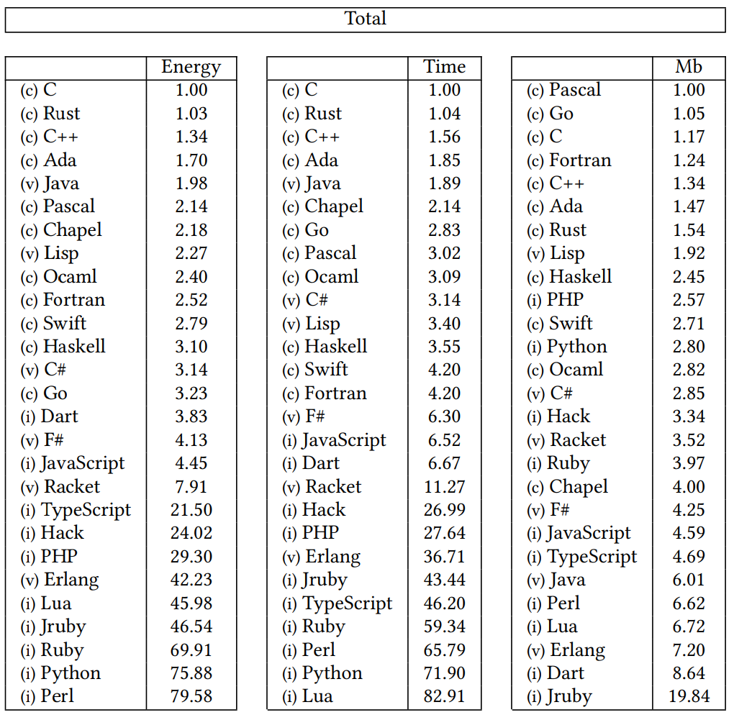
\includegraphics[width=\textwidth]{images/chapter_4_implementation/programming_language_comparison}
    \centering~\caption{A comparison of programming languages based on energy usage, time and memory
    efficiency\cite{programming_language_efficiency}.}
    \label{fig:chapter_4_implementation-programming_language_comparison}
\end{figure}

Although languages such as C and C++ outperform Java across all metrics displayed by
Figure~\ref{fig:chapter_4_implementation-programming_language_comparison}, they are needlessly low-level to the point
where it would likely become a hindrance. Even a cursory investigation into the nature of socket programming in C++
revealed a perfect case study as to the benefits of Java for a problem statement like Packet Courier's. It turns out
that Windows does not natively support the standard C++ socket specification, \texttt{sys/socket.h}, meaning that
\texttt{winsock2.h} must be used instead\cite{socket_vs_winsock}. This would then mean either going to the effort of
implementing two different platform-dependent solutions, or using a library that promises platform agnosticism. There
are many such libraries however\cite{c++_socket_libraries}, placing a substantial research burden on the development
of what should be a fairly simple component. C++ furthermore has been shown to have several non-trivial cross-platform
and cross-compiler discrepancies for even the most basic code\cite{c++_cross_compiler_differences,
    c++_statistical_differences, c++_random_differences, c++_filesystem_differences}.

A key benefit of Java is that it smooths out cross-platform issues, providing developers with a clean, uniform and
highly reliable set of semantics that transcend the nuances of the native operating system and hardware
micro-architecture. Indeed, Java handily has a \texttt{DatagramSocket} class\cite{java_DatagramSocket} which has
proven extremely useful in implementing Packet Courier's standalone emulator. In this way, external Java libraries
are only called-in for more heavyweight or highly specific work, as opposed to routine or menial implementations.

Java also strikes a Goldilocks-esque balance\cite{goldilocks_effect} between low-level languages like C++ and
languages that are arguably even more abstract than Java, such as Python. Whilst Packet Courier does leverage Python
3\cite{python_3} for basic client-server scripts to demonstrate the functionality of the emulator, production code
consists exclusively of Java. Python's dynamic typing\cite{python_typing}, poor
performance\cite{programming_language_efficiency} and inefficient multi-threading and synchronisation
primitives\cite{python_gil} are the main reasons why it wasn't used more prominently within Packet Courier.

\subsection{Build Management and Dependencies}

\subsubsection{JUnit 4}

TODO

\subsubsection{AssertJ}

TODO

\subsubsection{Google Protobuf}

TODO

\subsubsection{Protocol Buffers Protobuf Maven Plugin}

TODO

\subsection{Continuous Integration}

TODO


\section{API Overview}

\subsection{Repository Structure}

TODO

\subsection{Statistical Distribution API}

TODO

\subsection{Network Condition API}

TODO

\subsection{Worker API}

TODO

\subsection{Node API}

TODO

\subsection{Mail API}

TODO

\subsection{Simulation API}

TODO

\subsection{Miscilaneous}

TODO


\section{Standalone Emulator}

\subsection{Key Components}

TODO

\subsection{Protobuf Integration}

TODO


\section{Debugging Features}

\subsection{Process Monitor}

TODO

\subsection{Crash Dumps}

TODO

\subsection{Meta Logging}

TODO
